\documentclass[11pt]{article}
%Gummi|061|=)
\usepackage{amsmath}
\DeclareMathOperator*{\argmax}{arg\,max}
\title{\textbf{A Tour on EM Algorithm}}
\author{Tianxing He}
\date{}
\usepackage{graphicx}
\usepackage[top=1in, bottom=1in, left=1in, right=1in]{geometry}
\begin{document}
\bibliographystyle{plain}
\maketitle

\section{Introduction}
Since its formal introduction in 1977 by Dempster et al. \cite{ADempsterEM}, the EM algorithm has become a standard methodology for ML estimation. It has steadily become more and more popular and is being used in an increasing number of applications. The first publications in IEEE journals making reference to the EM algorithm appeared in 1988 and dealt with the problem of tomographic reconstruction of photon limited images \cite{1977Posit}, \cite{1988Bayes}. Since then, the EM algorithm has become a popular tool for statistical signal processing used in a wide range of applications, such as recovery and segmentation of images and video, image modelling, carrier frequency synchronization, and channel estimation in communications and speech recognition\cite{EMExtensions}. \\
Assume that x are the observations and $\theta$ the unknown parameters of a model that generated x. The ML estimate is obtained as 
\begin{equation}
\hat{\theta}_{ML}= \argmax_{\theta}L(\theta) = ln(p(x;\theta))
\end{equation}
However, in many cases the likelihood function $p(x;\theta)$ is complex and is either difficult or immpossible to directly optimize. In such cases the computation of this likelihood is greatly facilitated by the introduction of hidden variables z. These random variables act as links that connect the observations to the unknown parameters via Bayes’ law. The choice of hidden variables is problem dependent. However, as their name suggests, these variables are not observed and they provide enough information about the observations so that the conditional probability $p(x|z)$ is easy to compute. Apart from this role, hidden variables play
another role in statistical modeling. They are an important part of the probabilistic mechanism that is assumed to have generated the observations and can be described very succinctly by a graph that is termed “graphical model.” 
Once hidden variables and a prior probability for them $p(z;\theta)$ have been introduced, one can obtain the likelihood or the marginal likelihood as it is called at times by integrating
out (marginalizing) the hidden variables according to
\begin{equation}{\label{2}}
L(\theta) = lnp(x;\theta) = ln \int p(x,z;\theta) = ln \int P(x|z;\theta)p(z;\theta) 
\end{equation}
Despite the simplicity of the above formulation, in most cases of interest the integral in (\ref{2}) is either impossible or very difficult to compute in closed form. Thus, the main effort in Bayesian Inference is concentrated on techniques that allow us to bypass or approximately evaluate this integral.  \\
Such methods can be classified into two broad categories\cite{LifeAfter}. The first is numerical sampling methods also known as Monte Carlo techniques and the second is deterministic approximations. Here we won't address Monte Carlo methods\cite{2003MC}, \cite{MCMC}. On the other hand, the EM algorithm is a Bayesian inference methodology that assumes knowledge of the posterior $p(z|x;\theta)$ and iteratively maximizes the likelihood function without explicitly computing it.\\
One of the most insightful explanations of EM, that provides a deeper understanding of its operation than the intuition of alternating between variables, is in terms of lower-bound maximization \cite{neal}.\\
Assuming now we somehow have a parameter $\theta^{(p)}$, using JenSen's inequaility and following equation(\ref{2}), we have
\begin{equation}{\label{3}}
L(\theta) = ln \int P(x, z;\theta) = ln \int \frac{P(x, z;\theta)q(z)}{q(z)}
\geq \int q(z) ln\frac{P(x,z;\theta)}{q(z)}
\end{equation}
Where $q(z)$ could be any distribution. For EM Algorithm, we take $q(z) = p(z|x; \theta^{(p)})$, so
\begin{equation}
\begin{split}
\int q(z) ln\frac{P(x,z;\theta)}{q(z)} = \int p(z|x; \theta^{(p)}) ln\frac{P(x,z;\theta)}{p(z|x; \theta^{(p)})} \\ 
= \int p(z|x; \theta^{(p)}) lnP(x,z;\theta) - \int p(z|x; \theta^{(p)})lnp(z|x; \theta^{(p)})
\end{split}
\end{equation}
Notice the second term is constant. We now define the \textbf{auxiliary function}
\begin{equation}
Q(\theta, \theta^{(p)}) = \int p(z|x; \theta^{(p)}) lnP(x,z;\theta)
\end{equation}
Assume we have $\theta^{(p)}$, in the E-step, we deride the anxiliary function, then in the M-step, we maximize the anxiliary function to get $\theta^{(p+1)}$. One get the inituition of EM in equation (\ref{3}) : we are maximizing the lower bound of $L(\theta)$.
\begin{equation}
\begin{split}
&EM~Alorithm \\
E-Step &: compute~p(z|x;\theta^{old})\\
M-Step &: Evaluate~\theta^{new}=\argmax_{\theta}Q(\theta,\theta^{old})
\end{split}
\end{equation}
\section{Examples}
\subsection{Guassian Mixture Model}
The Guassian Mixture distribution is a linear superposition of Guassians: 
\begin{equation}
p(x) = \Sigma^K_{k=1}\pi_k\mathcal{N}(x|\mu_k,\Sigma_k)
\end{equation}
Subject to:
\begin{equation}
\Sigma^K_{k=1}\pi_k = 1
\end{equation}
\begin{figure}[htp]
\centering
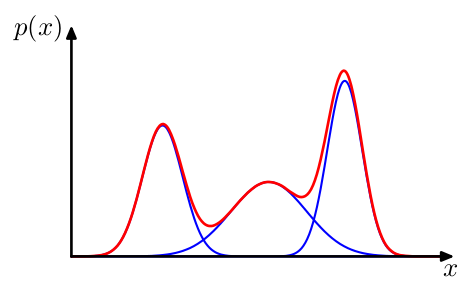
\includegraphics[scale=0.50]{GMM-example2.png}
\caption{The Guassian Mixture Model}
\end{figure}

Given a Guassian Mixture model, we introduce K-dimensional binary random variable z which only one element $z_k$ is euqal to 1 and the others are all 0.\\
\begin{equation}
z=(0,0,..,1,0,..0)
\end{equation}
So there are K possible states for z.And we let
\begin{equation}
p(z_k=1) = \pi_k
\end{equation}
That is to say, 
\begin{equation}
p(z) = \prod^K_{k=1}{\pi_k}^{z_k}
\end{equation}
Then, we define the conditional distribution of x given a particular z:
\begin{equation}
p(x|z_k=1)=\mathcal{N}(x|\mu_k,\Sigma_k)
\end{equation}
which can also be written as:
\begin{equation}
p(x|z)=\prod^K_{k=1}{\mathcal{N}(x|\mu_k,\Sigma_k)}^{z_k}
\end{equation}
Now we can easily compute the marginal distribution of x
\begin{displaymath}
\begin{split}
p(x) = \Sigma_zp(x|z)p(z) &= \Sigma_z\prod^K_{k=1}{\mathcal{N}(x|\mu_k,\Sigma_k)}^{z_k}
\prod^K_{k=1}{\pi_k}^{z_k}\\
 &=\Sigma^K_{k=1}\pi_k\mathcal{N}(x|\mu_k,\Sigma_k)
\end{split}
\end{displaymath}
\begin{figure}[htp]
\centering
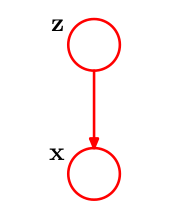
\includegraphics[scale=0.30]{latent-variable.png}
\caption{$p(x)=\Sigma_z p(x,z)$}
\label{}
\end{figure}
Now, instead of working with $p(x)$ we can work with $p(x,z) = p(x|z)p(z)$, which will lead to significant simplification when we are introducing the EM algorithm.\\
If we have a sequence of observances X, now we apply the EM algorithm.
\begin{equation}{\label{maxlike}}
lnp(X|\pi,\mu,\Sigma)=\Sigma^N_{n=1}ln\{\Sigma^K_{k=1}\pi_k
\mathcal{N}(x_n|\mu_k,\Sigma_k)\}
\end{equation}
Remembering the anxiliary function is
\begin{equation}
Q(\theta, \theta^{old}) = \int p(z|x; \theta^{old}) lnP(x,z;\theta)
\end{equation}
For GMM
\begin{equation}
Q(\theta, \theta^{old}) = \Sigma_Z p(Z|X, \theta^{old}) ln p(X,Z|\theta)
\end{equation}
Z is a vector of length N, indicating which Guassian component each observance is from.\\ For GMM, we have the constraint that $\Sigma \pi_i = 1$, using the lagrange multiplier, we should maximize
\begin{equation}
\Lambda = \Sigma_Z p(Z|X, \theta^{old}) ln p(X,Z|\theta) + \lambda(\Sigma_k \pi_k - 1)
\end{equation}
Now we set the derivative of each variable to zero:
\begin{equation}
\frac{\partial \Lambda}{\partial \lambda} = \Sigma_k \pi_k -1=0
\end{equation}
For simplicity,  we consider each $x_i$, which means, we consider $lnp(X,Z|\theta)$ as $\Sigma_i ln(p(x_i,z_i))$, unfold, and look at each $i$. Because the sequence is generated independently, the term$p(Z|X,\theta^{old})$ can be regarded as $Const * \gamma(z_{ik})$.
\begin{equation}
\begin{split}
\frac{\partial \Lambda}{\partial \pi_k} &= \frac{Const* \partial ln(\pi_k)\Sigma_i\gamma(z_{ik}) + \lambda \pi_k}{\partial \pi_k}\\
&=\frac{1}{\pi_k}\Sigma_i\gamma(z_{ik})+\lambda=0
\end{split}
\end{equation}
\begin{equation}
\begin{split}
\frac{\partial \Lambda}{\partial \mu_k} &= \frac{Const* \Sigma_i \gamma(z_{ik}) \partial (-1/2 * (x_i-\mu_k)^T\Sigma_k^{-1}(x_i-\mu_k)) }{\partial \mu_k}\\
&= Const * \Sigma_i \gamma(z_{ik})\frac{-1}{2}((x_i-u_k)^T\Sigma_k^{-1}+\Sigma_k^{-1}(x_i-\mu_k))\\
&= Const * \Sigma_i \gamma(z_{ik})((x_i-\mu_k)^T\Sigma_k^{-1})=0
\end{split}
\end{equation}
Note that in the second step we use a constraint that $\Sigma$ is symmetric, so is $\Sigma^{-1}$.\\
The derivation for $\partial \Sigma$ is more complex, we need to use some conclusion from Appendix A. Now we can get the update formula for each variable by solving these equations:\\
 \textbf{E-step} Evaluate the responsibilities using the current parameter values.
\begin{equation}
\begin{split}
\gamma (z_{nk}) = \frac{\mathcal{N}(x_n|\mu_k, \Sigma_k)}{\Sigma^K_{k=1}\pi_k\mathcal{N}(x_n|\mu_k,\Sigma_k)}
\end{split}
\end{equation}
\textbf{M-step} 
Re-estimate the parameters using the current responsibilities.
\begin{equation}
\begin{split}
\mu_k^{new}&=\frac{1}{N_k}{\Sigma^{N}_{n=1}\gamma(z_{nk})x_n}\\
\Sigma_k^{new}&=\frac{1}{N_k}\gamma_k(z_{nk})(x_n-\mu_k)(x_n-\mu_k)^T\\
\pi_k^{new}&=\frac{N_k}{N}
\end{split}
\end{equation}
\textbf{Likelihood} Recalculate the log likelihood function to see if it converges, if not, go to step 1 again.
Where
\begin{equation}
N_k=\Sigma_i\gamma(z_{ik})
\end{equation}

\subsection{HMM-GMM in ASR}
\subsubsection{Introduce the HMM-GMM model}
New machine learning algorithms can lead to significant advances in automatic speech recognition(ASR).The biggest advance occurred nearly four decades ago with the introduction of the EM algorithm for training HMMs\cite{HMM1}. Most current speech recognition systems\cite{DNN1} use hidden Markov models to deal with the temporal variability of speech and Gaussian mixture models(GMM) to determine how well each state of each HMM fits a frame or a short window of frames of coefficients that represents the acoustic input. An alternative way to evaluate the fit is to use a feed-forward neural network that takes several frames of coefficients as input and
produces posterior porbabilities over HMM states as output. GMMs have a number of advantages that make them suitable for modeling the probability distributions over vectors of input features that are associated with each state of an HMM. With enough components, they can model probability distributions to any required level of accuracy, and they are fairly easy to fit to data using the EM algorithm. \\
Despite all their advantages, GMMs have a serious shortcomings. They are statistically\cite{HMM2} inefficient for modeling data that lie on or near a nonlinear manifold in the data space. For example, modeling the set of points that lie very close to the surface of a sphere only requires a few parameters using an appropriate model class, but it requires a very large number of diagonal Gaussians or a fairly large number of full-covariance Gaussians. Speech is produced by modulating a relatively small number of parameters of a dynamical system, and this implies that its true underlying structure is much lower-dimensional than is immediately apparent in a window that contains hundreds of coefficients. It is believed, therefore, that other types of model may work better than GMMs for acoustic modeling if they can more effectively exploit information embedded in a large window of frames.\\
\begin{figure}
\centering
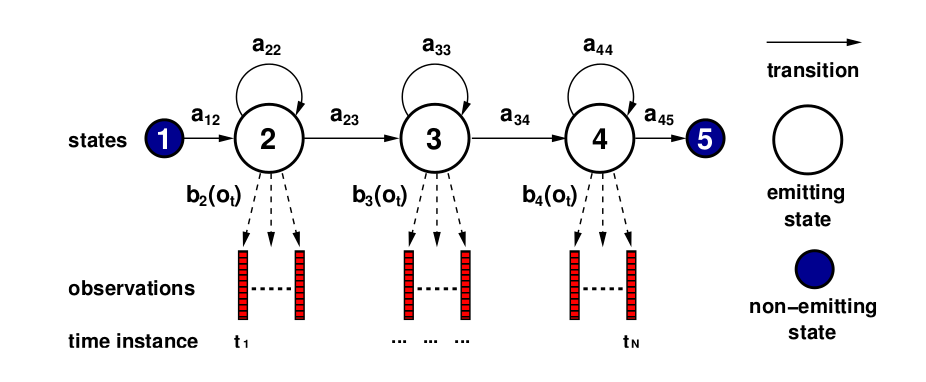
\includegraphics[width=300pt]{HMM.png}
\caption{The HMM-GMM model}
\end{figure}
We use a HMM to model a \emph{context dependent phone}. $a_{ij}$ is the state transition probability. $b(o)$ is a single Guassian distribution that models the observance that this state.\\
We call $O=(o_1,o_2,...,o_T)$ the observance of a HMM, and $w = (w_1,w_2,...,w_T)$ the hidden state sequence.
\subsubsection{Apply the EM algorithm}
We will now assume that $b(o)$ is Guassian (instead of Guassian Mixture) for simplicity.
As before, we unfold the anxiliary function.
\begin{equation}
\begin{split}
Q_{ML}(M_{k+1};\hat{M}_{k}) = \sum_w logp(O,w|M_{k+1})p(w|O,\hat{M}_k) \\
                            = \sum_w log(a_{w_0w_1}\prod_ta_{w_{t-1}w_t}b_{w_t}(o_t)) P(w|O, \hat{M}_k) \\
Q_{ML}(M_{k+1};\hat{M}_{k}) = \sum_{t,j} \gamma_j(t)logb_j(o_t)+\sum_{t,i,j}\varepsilon_{ij}(t)loga_{ij}
\end{split}                 
\end{equation}
Where $\gamma_j(t) = P(w_t=j|O,\hat{M}_k)$ and $\varepsilon_{ij}(t) = P(w_{t-1}=i,w_t=j|O,\hat{M}_k)$. And the transistion is simply via take each $a$ and $b$ out and add all out their cooresponding $w$.\\
To calculate $\gamma_j$ and $\varepsilon_{ij}$, we need to calculate $\alpha_j(t) = p(o_{1-t}, w_t=j|\hat{M}_k)$ and $\beta_j(t)=p(o_{t+1-T}|w_t=j, \hat{M}_k)$
They can be calculated efficiently:
\begin{equation}
\begin{split}
\alpha_j(t) = (\sum_{i=2}^{N-1}\alpha_i(t-1)a_{ij})b_j(o_t) \\
\beta_j(t) = \sum_{i=2}^{N-1}a_{ji}b_i(o_{t+1})\beta_i(t+1)
\end{split}
\end{equation}
Then we have
\begin{equation}
\begin{split}
\gamma_j(t) &= \frac{\alpha_j(t) \beta_j(t)}{p(O|\hat{M}_k)} \\ 
\varepsilon_{ij}(t) &= \frac{\alpha_i(t-1) a_{ij} b_j(o_t) \beta_j(t)}{p(O|\hat{M}_k)}
\end{split}
\end{equation}
Having got the $\gamma$ and $\varepsilon$, we finally could try to maximize 
\begin{equation}
Q_{ML}(M_{k+1};\hat{M}_{k}) = \sum_{t,j} \gamma_j(t)logb_j(o_t)+\sum_{t,i,j}\varepsilon_{ij}(t)loga_{ij}
\end{equation}
First let's consider $a_{i*}$, now we should maxmize $\sum_{t,j} \varepsilon_{ij}(t)loga_{ij}$ subject to $\sum_j a_{ij} = 1$, we could use the lagrange multiplier, I omit the derivation here.
\begin{equation}
\hat{a}_{ij} = \frac{\sum^{T}_{t=2}\varepsilon_{ij}(t)}{\sum^{T}_{t=1}\gamma_i(t)}
\end{equation}
Now we maximize the other component $\sum_{t,j} \gamma_j(t)logb_j(o_t)$.We set $G(\mu_j, \Sigma_j) = \sum_{t} \gamma_j(t)logb_j(o_t)$. And we maximize it by solving $\frac{\partial G}{\partial \mu_j}=0$. Then we get,
\begin{equation}
\hat{\mu_j} = \frac{\sum_t(\gamma_j(t)o_t)}{\sum_t\gamma_j(t)}
\end{equation}

%%%%%%%%%%%%%%%%%%%%%%%%%%%%%%%%%%%%%%%%%%%%%%%%%%%%%%%%%%%%%%%%%%%%%%%%%%%%%%%%%%%%%%%%%%%
\section{Properities of the EM algorithm}
\subsection{Monotonous Increase of the Likelihood}
We follow the exposition of the EM in \cite{PRML} and \cite{1998RM}. It is straightforward to show that the log-likelihood can be written as
\begin{equation}{\label{4}}
lnp(x;\theta)=F(q,\theta) + KL(q||p)
\end{equation}
where
\begin{equation}
F(q,\theta)=\int q(z)ln\frac{p(x,z;\theta)}{q(z)}
\end{equation}
and
\begin{equation}
KL(q||p)=\int -q(z)ln\frac{p(z|x;\theta)}{q(z)}
\end{equation}
Notice that we always have $KL(q||p) \geq 0$ as long as $q$ is a distribution.\\
Now, assuming we have a $\theta^{(p)}$, and let $q(z) = p(z|x;\theta^{(p)})$, we can get $\theta^{(p+1)}$ through an iteration:
\begin{equation}
\theta^{(p+1)} = \argmax_{\theta}F(q, \theta)
\end{equation}
Notice this is equal to maximizing the anxiliary function.\\
Now, one can easily find out that if we just take $\theta^{(p+1)}=\theta^{(p)}$, we have$F(q, \theta^{(p+1)}) = L(\theta^{(p)})$, because $KL(q||p)=0$. Since we are maximizing $F$, we have
\begin{equation}
F(q, \theta^{(p+1)}) \geq L(\theta^{(p)})
\end{equation}
Remembering that we always have $KL(q||p) \geq 0$, we get
\begin{equation}
L(\theta^{(p+1)}) \geq L(\theta^{(p)})
\end{equation}	
\subsection{Convergence to a Local Maxima}
With the exception of a few specific cases, the EM algorithm is not guaranteed to converge to a global maximizer of the likehood\cite{EMTour, Xu95onconvergence}. Under some regularity conditions on the likelihood $L(\theta)$ and on the parameters set $\Theta$, it is possible, however, to show the parameter sequence obtained by EM converges to a local maximizer of $L(\theta)$ or at least, to a stationary point of $L(\theta)$. Necessary conditions for the convergence of the EM algorithm and related theorems can be found in \cite{EMCov}.
\section{Variants of the EM Algorithm}
\subsection{Penalized Likelihood Estimation}
The EM algorithm can be straightforwardly modified to compute penalized likelihood estimates, that is, estimates of the form
\begin{equation}
\theta = \argmax_{\theta}[L(\theta)+G(\theta)]
\end{equation}
The penalty term $G(\theta)$ could represent, for example, the logarithm of a prior on if a Bayesian approach is used and the maximum a posteriori(MAP) estimate of is desired instead of the ML estimate.(Someone put it "poor man’s bayesian inference\cite{LifeAfter}") The EM algorithm for penalized-likelihood estimation can be obtained by replacing the M-step with
\begin{equation}
\theta^{(p+1)}=\argmax_{\theta}[Q(\theta, \theta^{(p)}) +G(\theta)]
\end{equation}
It is straightforward to see that the monotonicity property is preserved. Examples of penalized likelihood estimation to be found in \cite{penalized}.
\subsection{Variational EM}
One can bypass the requirement of exactly knowing $p(z|x;\theta)$ by assuming an appropriate q(z) in the decomposition (\ref{4})\cite{LifeAfter}. In the E-step q(z) is found such that it maximizes $F(q,\theta)$ keeping $\theta$ fixed. To perform this maximization, a particular
form of q(z) must be assumed. In certain cases it is possible to assume knowledge of the form of $q(z;\omega)$, where ω is a set of ω parameters. Thus, the lower bound $F(\omega,\theta)$ becomes a function of these parameters and is maximized with respect to ω in the E-step and with respect to θ in the M-step. The process can be summarized as below\cite{gentle}:
\begin{equation}
\begin{split}
&Variational~EM \\
Variational~E-Step &: compute~\hat{q} = \argmax_{q}F(q, \theta^{old})\\
Variational~M-Step &: Evaluate~\theta^{new}=\argmax_{\theta}F(\hat{q},\theta)
\end{split}
\end{equation}
One can easily deduce the monotonicity property is still preserved, since we can first prove
\begin{equation}
F(\hat{q},\theta^{old}) \geq L(\theta^{old})
\end{equation}
and then
\begin{equation}
F(\hat{q}, \theta^{new}) \geq F(\hat{q}, \theta^{old})
\end{equation}
because of the {argmax}.\\
Although there are no approximations in the variational theory, variational methods can be used to find approximate solutions in Bayesian inference problems. This is done by assuming that the functions over which optimization is performed have specific forms. For example, we can assume only quadratic functions or functions that are linear combinations of fixed basis functions. For Bayesian inference, a particular form that has been used with great success is the factorized one, see \cite{1var} and \cite{2var}. In which case we assume
\begin{equation}
q(z)=\prod^{M}_{i=1}q_i(z_i)
\end{equation} 
From that assumption we could deride \cite{LifeAfter}
\begin{equation}
q_j^*(z_j)=\frac{exp(<lnp(x,z;\theta)>_{i\neq j})}{\int exp(<lnp(x,z;\theta)>_{i\neq j})dz_j}
\end{equation}

\section{Appendix}
\subsection{A:The derivative of the Guassian likelihood with respect to covariance matrix}
First we list some math tools we will use:
\begin{equation}
\frac{\partial}{\partial A}ln|A|=(A^{-1})^T 
\end{equation}
\begin{equation}
\frac{\partial[X^{-1}A]}{\partial X}=-X^{-1}A^TX^{-1}
\end{equation}

We have the Guassian likelihood:
\begin{equation}
ln(\mathcal{N}(x|\mu, \Sigma))=-\frac{D}{2}ln(2\pi) + (-\frac{1}{2})ln(|\Sigma|) + (-\frac{1}{2})(x-\mu)^T\Sigma^{-1}(x-\mu)
\end{equation}
Now we differentiate it with respect to $\Sigma$, we get
\begin{equation}
\begin{split}
\frac{\partial ln(\mathcal{N}(x|\mu, \Sigma))}{\partial \Sigma}&= {\Sigma}^{-1} + \frac{\partial Tr[\Sigma^{-1}(x-\mu)(x-\mu)^T]}{\partial \Sigma} \\
&= {\Sigma}^{-1} -\Sigma^{-1}(x-\mu)(x-\mu)^T\Sigma^{-1}
\end{split}
\end{equation}
By setting the derivative to zero, we get 
\begin{equation}
\Sigma=(x-\mu)(x-\mu)^T
\end{equation}

\bibliography{ref}

\end{document}
